\section{Kerberos}

In un sistema si può aggiungere una procedura di autenticazione per ogni servizio,
ad esempio una password per accedere al sistema, una per accedere al file system,
ecc. Questa tecnica risulta essere molto scomoda, soprattutto se si utilizzano
i token. Un’alternativa consiste nell’utilizzare un’unica credenziale di
autenticazione per accedere a tutti i servizi; avere un’unica password è una
soluzione comoda ma poco robusta.
Kerberos è un \textbf{protocollo} reale che si occupa di questo problema (e non solo),
ha come obiettivo quello di garantire la segretezza, l’autenticità
(ad accesso singolo), la temporalità (le chiavi usate hanno validità limitata
per prevenire \textit{replay attack}).
Quest’ultima caratteristica viene gestita tramite
i \textbf{timestamp}. In pratica, l’accesso ad un servizio avviene tramite
“biglietto” che vale per un periodo limitato; anche se tale biglietto venisse
intercettato, può essere usato solo una volta e per un breve tempo.

\paragraph{Kerberos}
è un protocollo di autenticazione dei servizi di rete creato dal MIT che si
serve della crittografia a chiave simmetrica per autenticare gli utenti per i
servizi di rete, eliminando così la necessità di inviare le password attraverso
la rete. Ricorre ad un’unica credenziale di autenticazione per accedere a tutti
i servizi. L'autenticazione mediante Kerberos impedisce agli utenti non autorizzati
di intercettare le password inviate attraverso la rete.
Il nome Kerberos deriva da Cerbero, il cane a tre teste che sorveglia
le porte dell’Ade.\\

La maggior parte dei sistemi di rete convenzionali usa uno schema di
autenticazione basato sulle password. Quando un utente effettua una
autenticazione per accedere ad un server di rete deve fornire le credenziali.
Sfortunatamente, la trasmissione delle informazioni di autenticazione spesso
non è criptata. Per essere sicuri, la rete non deve essere accessibile
dall'esterno e tutti i computer e gli utente sulla rete devono essere fidati.
Anche una volta che una rete è collegata a Internet, non si potrà più assumere
che la rete sia sicura, in quanto qualunque aggressore che ha accesso alla rete
può intercettare le password e i nomi utente che la attraversano.
Lo scopo principale di Kerberos è quello di eliminare la trasmissione delle
informazioni di autenticazione attraverso la rete.
Il suo corretto utilizzo permette di ridurre drasticamente la possibilità di
intercettazione. Per funzionare, Kerberos deve avere possedere due requisiti:

\begin{itemize}
    \item un \textbf{timeserver} in ogni sistema dove viene utilizzato.
          I timestamp permettono di sincronizzare le macchine;
    \item ogni utente deve avere una \textbf{chiave pubblica} e una \textbf{privata}
          (una password a lungo termine).

\end{itemize}

\subsection{Come funziona ?}

L’utente, una volta entrato nella propria macchina, vuole accedere ai servizi
messi a disposizione nella rete. Supponiamo voglia raggiungere il server in basso.
Effettuato il primo accesso alla macchina, le credenziali dell’utente vengono
inviate ad uno speciale servizio centrale, il Kerberos, che ricorre essenzialmente
a due tipi di server:

\begin{itemize}
    \item \textit{Authentication Server} (\textbf{AS}\footnote{Ricordarsi che
              AS non sta per
              \textit{Autonomous System} !}),
          che ha lo scopo di autenticare l’user;
    \item \textit{Ticket-Granting Server} (\textbf{TGS}), che a seconda dell’user,
          gli assegna i diritti per compiere determinate azioni;
\end{itemize}

\begin{figure}[H]
    \centering
    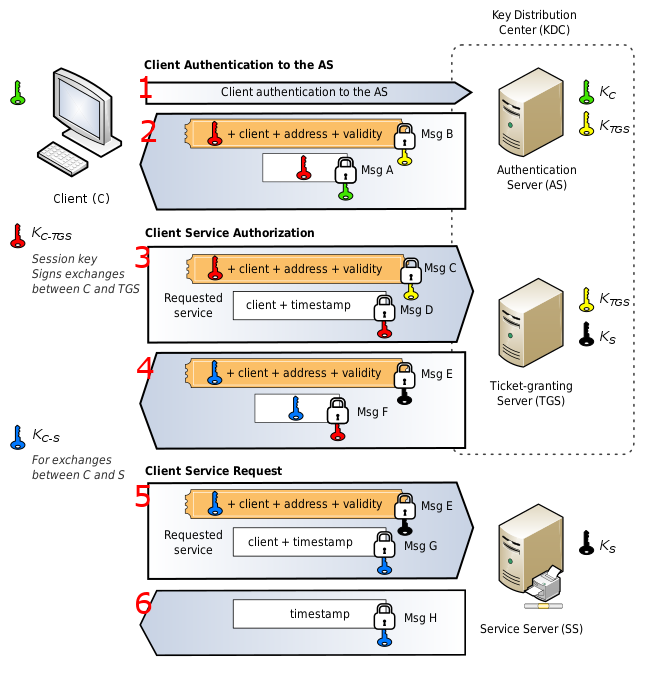
\includegraphics[width=10cm, keepaspectratio]{capitoli/autenticazione/imgs/kerberos1.png}
    \caption{Schema di funzionamento del protocollo Kerberos.}
\end{figure}

\begin{enumerate}
    \item L’utente si connette con le proprie credenziali alla workstation e
          queste vengono passate al Kerberos;
    \item AS verifica il diritto di accesso dell’utente, ricercando una
          corrispondenza nel database. Se il confronto ha esito positivo, AS
          assegna all’user un ticket e una session key.
          Il ticket verrà poi passato al TGS per richiedere i servizi, mentre
          la chiave permette di codificare le sue richieste, sempre poste al TGS.
          Entrambe le informazioni vengono criptate;
    \item L’utente a questo punto vuole utilizzare un certo servizio.
          La workstation richiede all'utente la password e la utilizza per
          decrittografare il messaggio in arrivo, quindi invia ticket e
          autenticatore
          (che contiene il nome, la rete, l'indirizzo e l'ora dell'utente) a TGS;
    \item TGS decripta il ticket e l'autenticatore, verifica se esso ha il
          diritto o meno ad utilizzare una certa risorsa e crea il ticket
          specifico per il servizio richiesto. La comunicazione tra utente e
          TGS avviene solo grazie alla session key che la codifica;
    \item La workstation manda ticket e autenticatore al server;
    \item Il server verifica il match tra ticket ed autenticatore e permette
          l’accesso al servizio. Se
          viene richiesta una mutua autenticazione, il server ritorna un
          autenticatore.
\end{enumerate}

È importante notare che l’utente può utilizzare il ticket finché esso risulta
ancora valido, il che può accadere anche per più tentativi di richiesta al servizio.
Per un servizio diverso mai utilizzato, deve ripercorrere il medesimo processo.\\

Kerberos opera fondamentalmente in \textbf{3 fasi}.

%% TODO: continuare da pagina 31